\subsection{Signal extraction procedure}
The two BDT classifiers introduced in the previous section, trained against the dominant \ttbar\ and \ttV\ backgrounds in each channel, are used to evaluate the limits in a fit to the classifier shape.
Figure~\ref{fig:mva12} shows the expected output distributions in a 2D plane of one training vs.\ the other.
Each event is now classified into one of ten 2D-bins according to its position in the plane, see Fig.~\ref{fig:binning}.
The number of bins is chosen such that no bins are entirely empty for any process.
The bin boundary positions have been studied and optimized with respect to the expected limit, see Sec.~\ref{sec:binopt}.

\begin{figure} [!h]
 \centering
 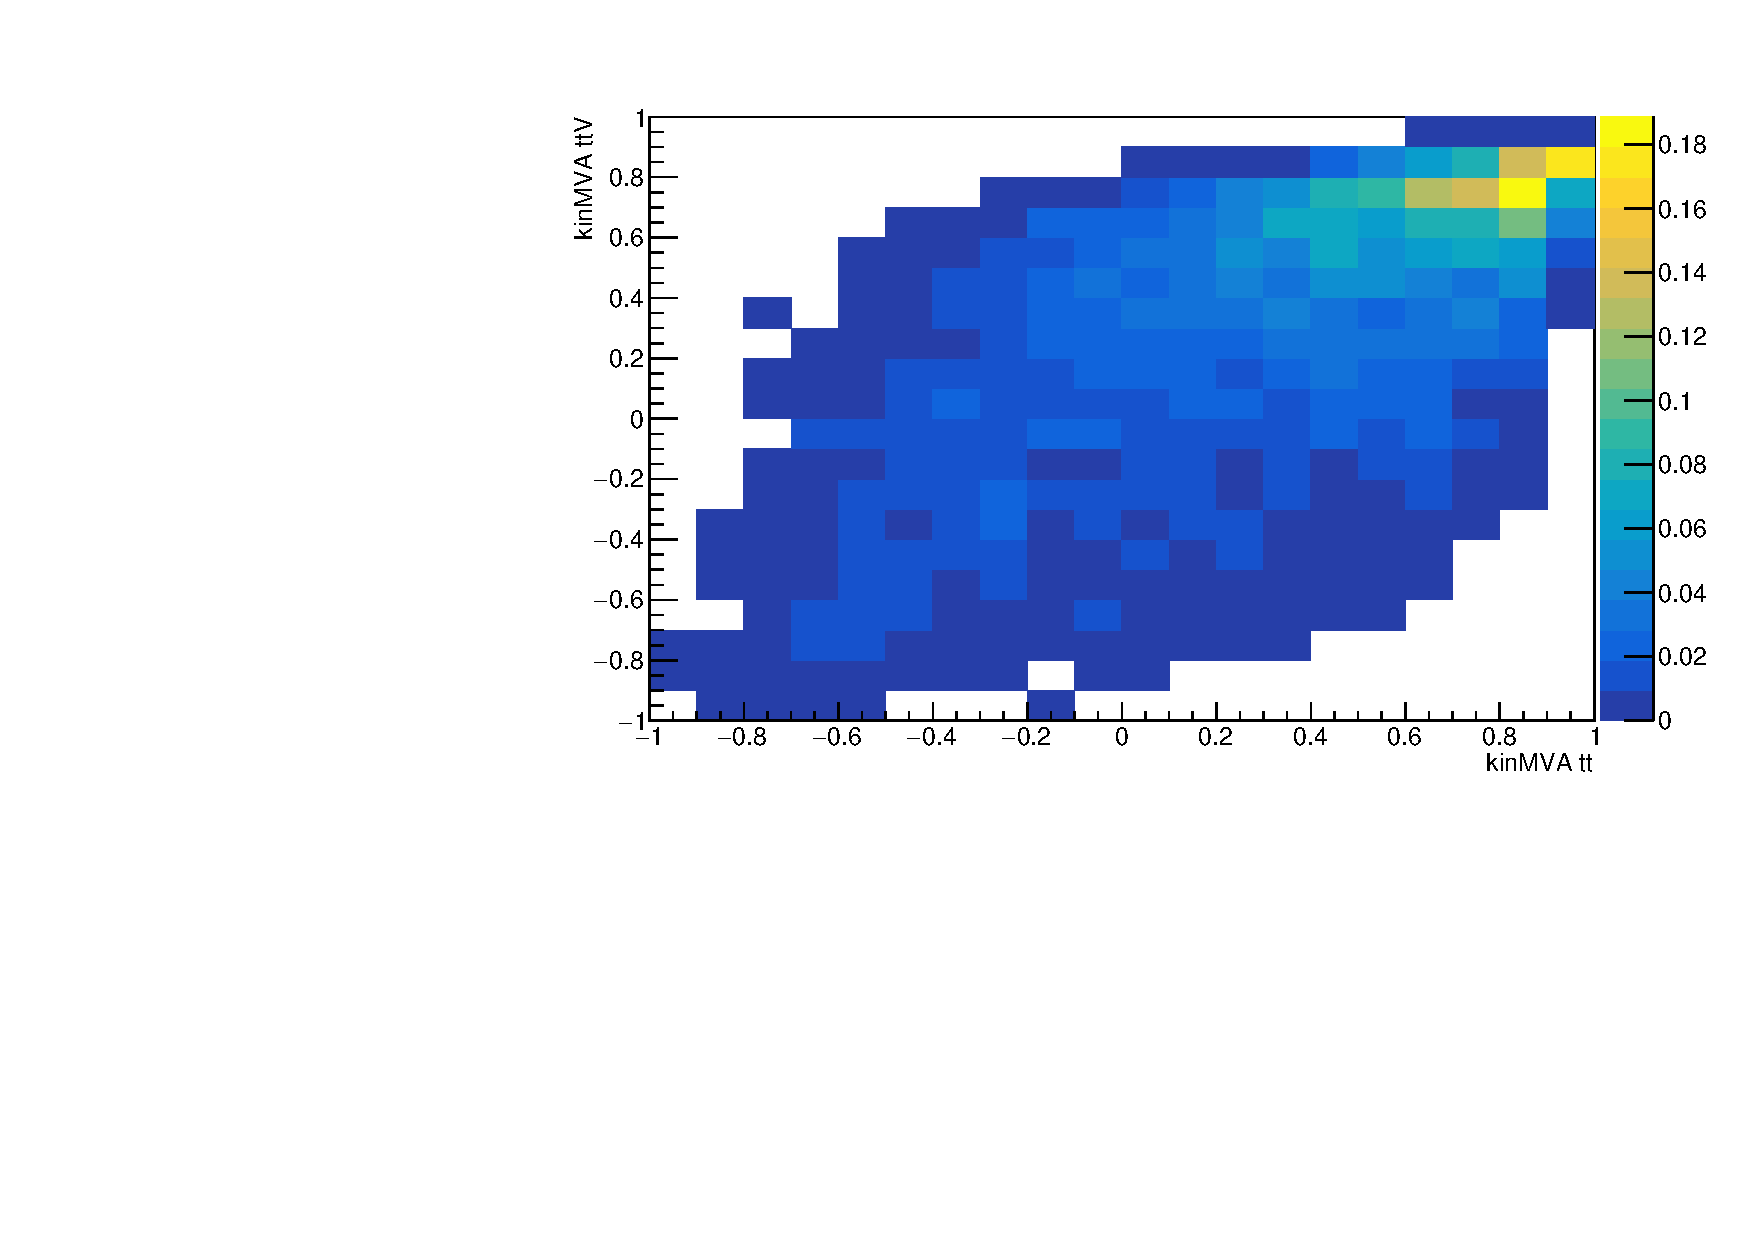
\includegraphics[width=0.45\textwidth]{figures/hthq.pdf}
 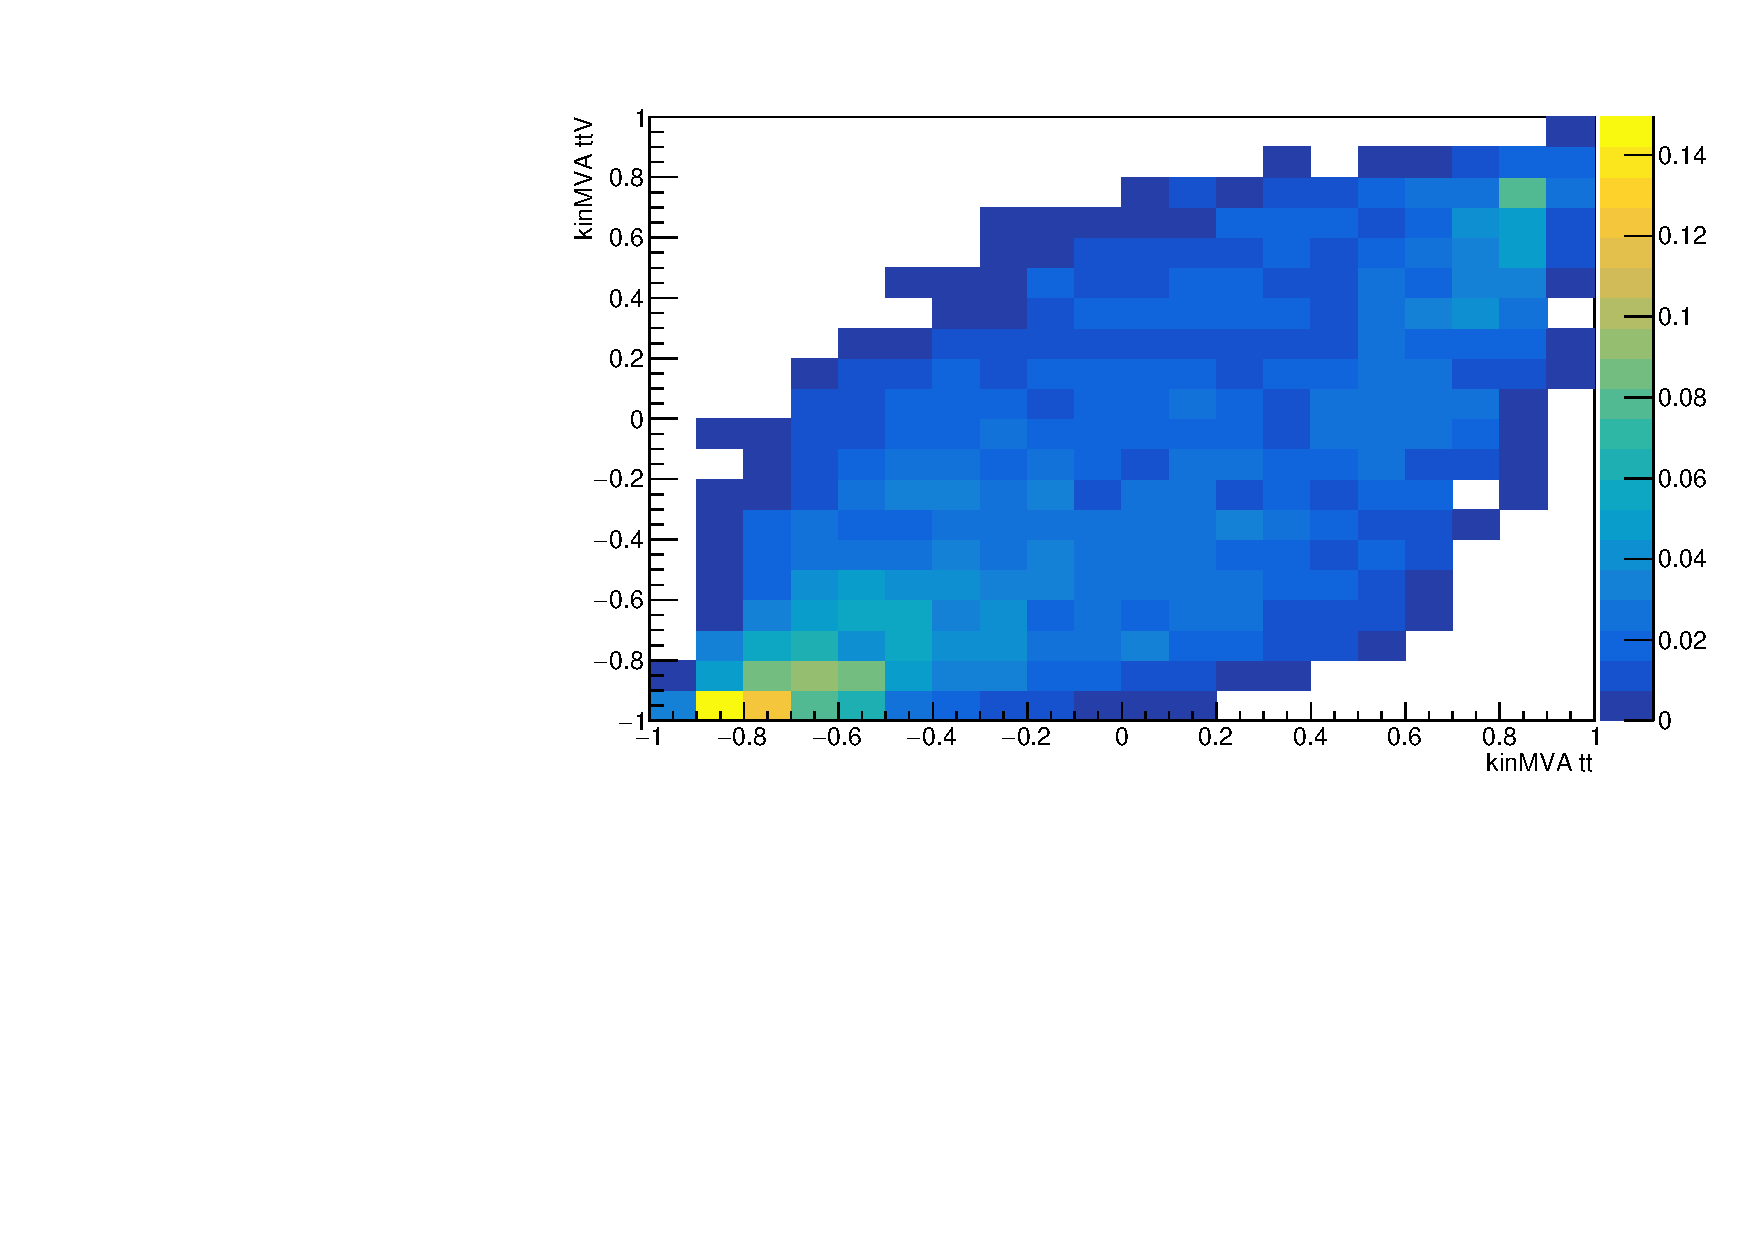
\includegraphics[width=0.45\textwidth]{figures/hthw.pdf}\\
 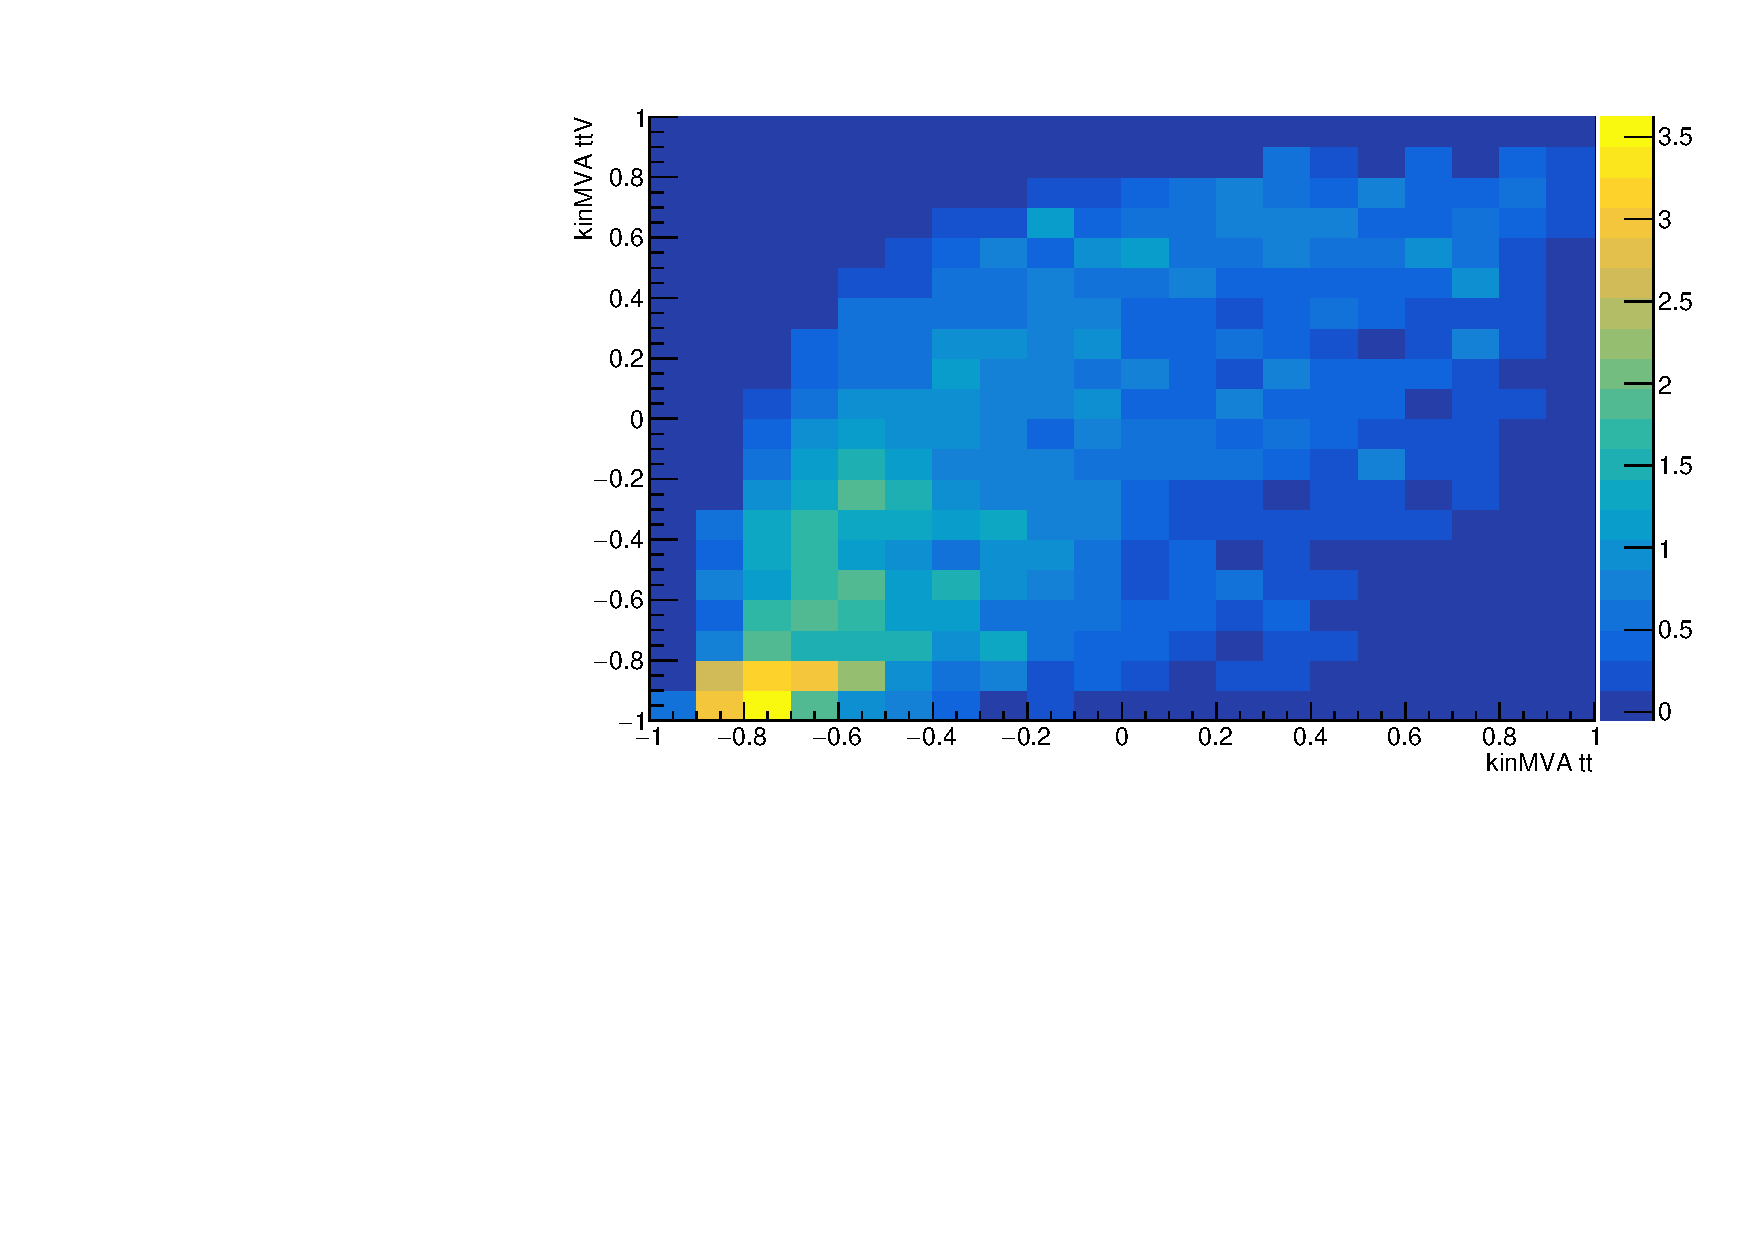
\includegraphics[width=0.45\textwidth]{figures/hbg.pdf}
 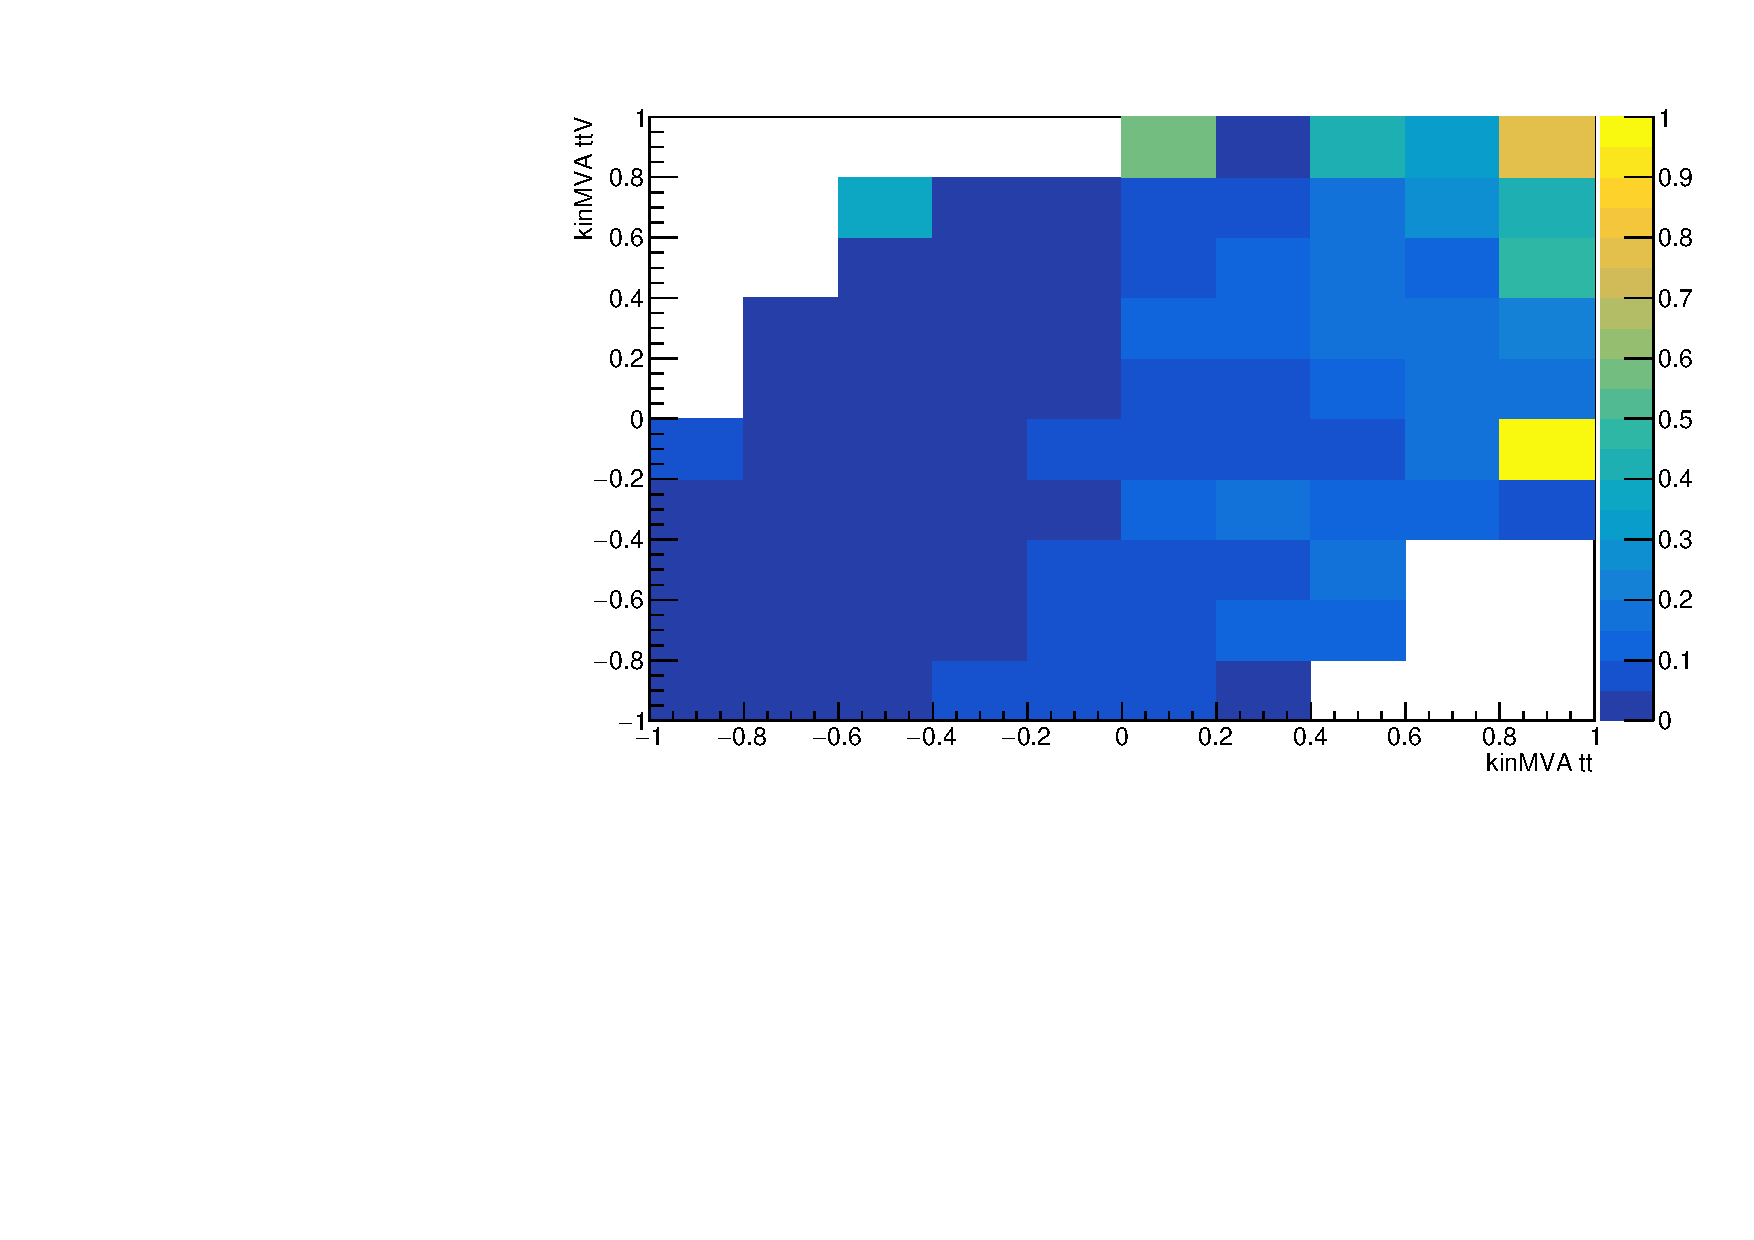
\includegraphics[width=0.45\textwidth]{figures/hratio.pdf}
\caption{BDT classifier output planes (training vs \ttbar\ on x-axis and vs \ttV\ on y-axis) for the \tHq\ and \tHW\ signals (top row), and for the combined backgrounds (bottom left). Backgrounds are evaluated as in the final background prediction, \ie\ these are not the samples used in the MVA training and this includes data-driven backgrounds. Bottom right shows the S/B ratio (combining \tHq\ and \tHW) in the same plane. Three lepton channel only.}
\label{fig:mva12}
\end{figure}

\begin{figure} [!h]
 \centering
 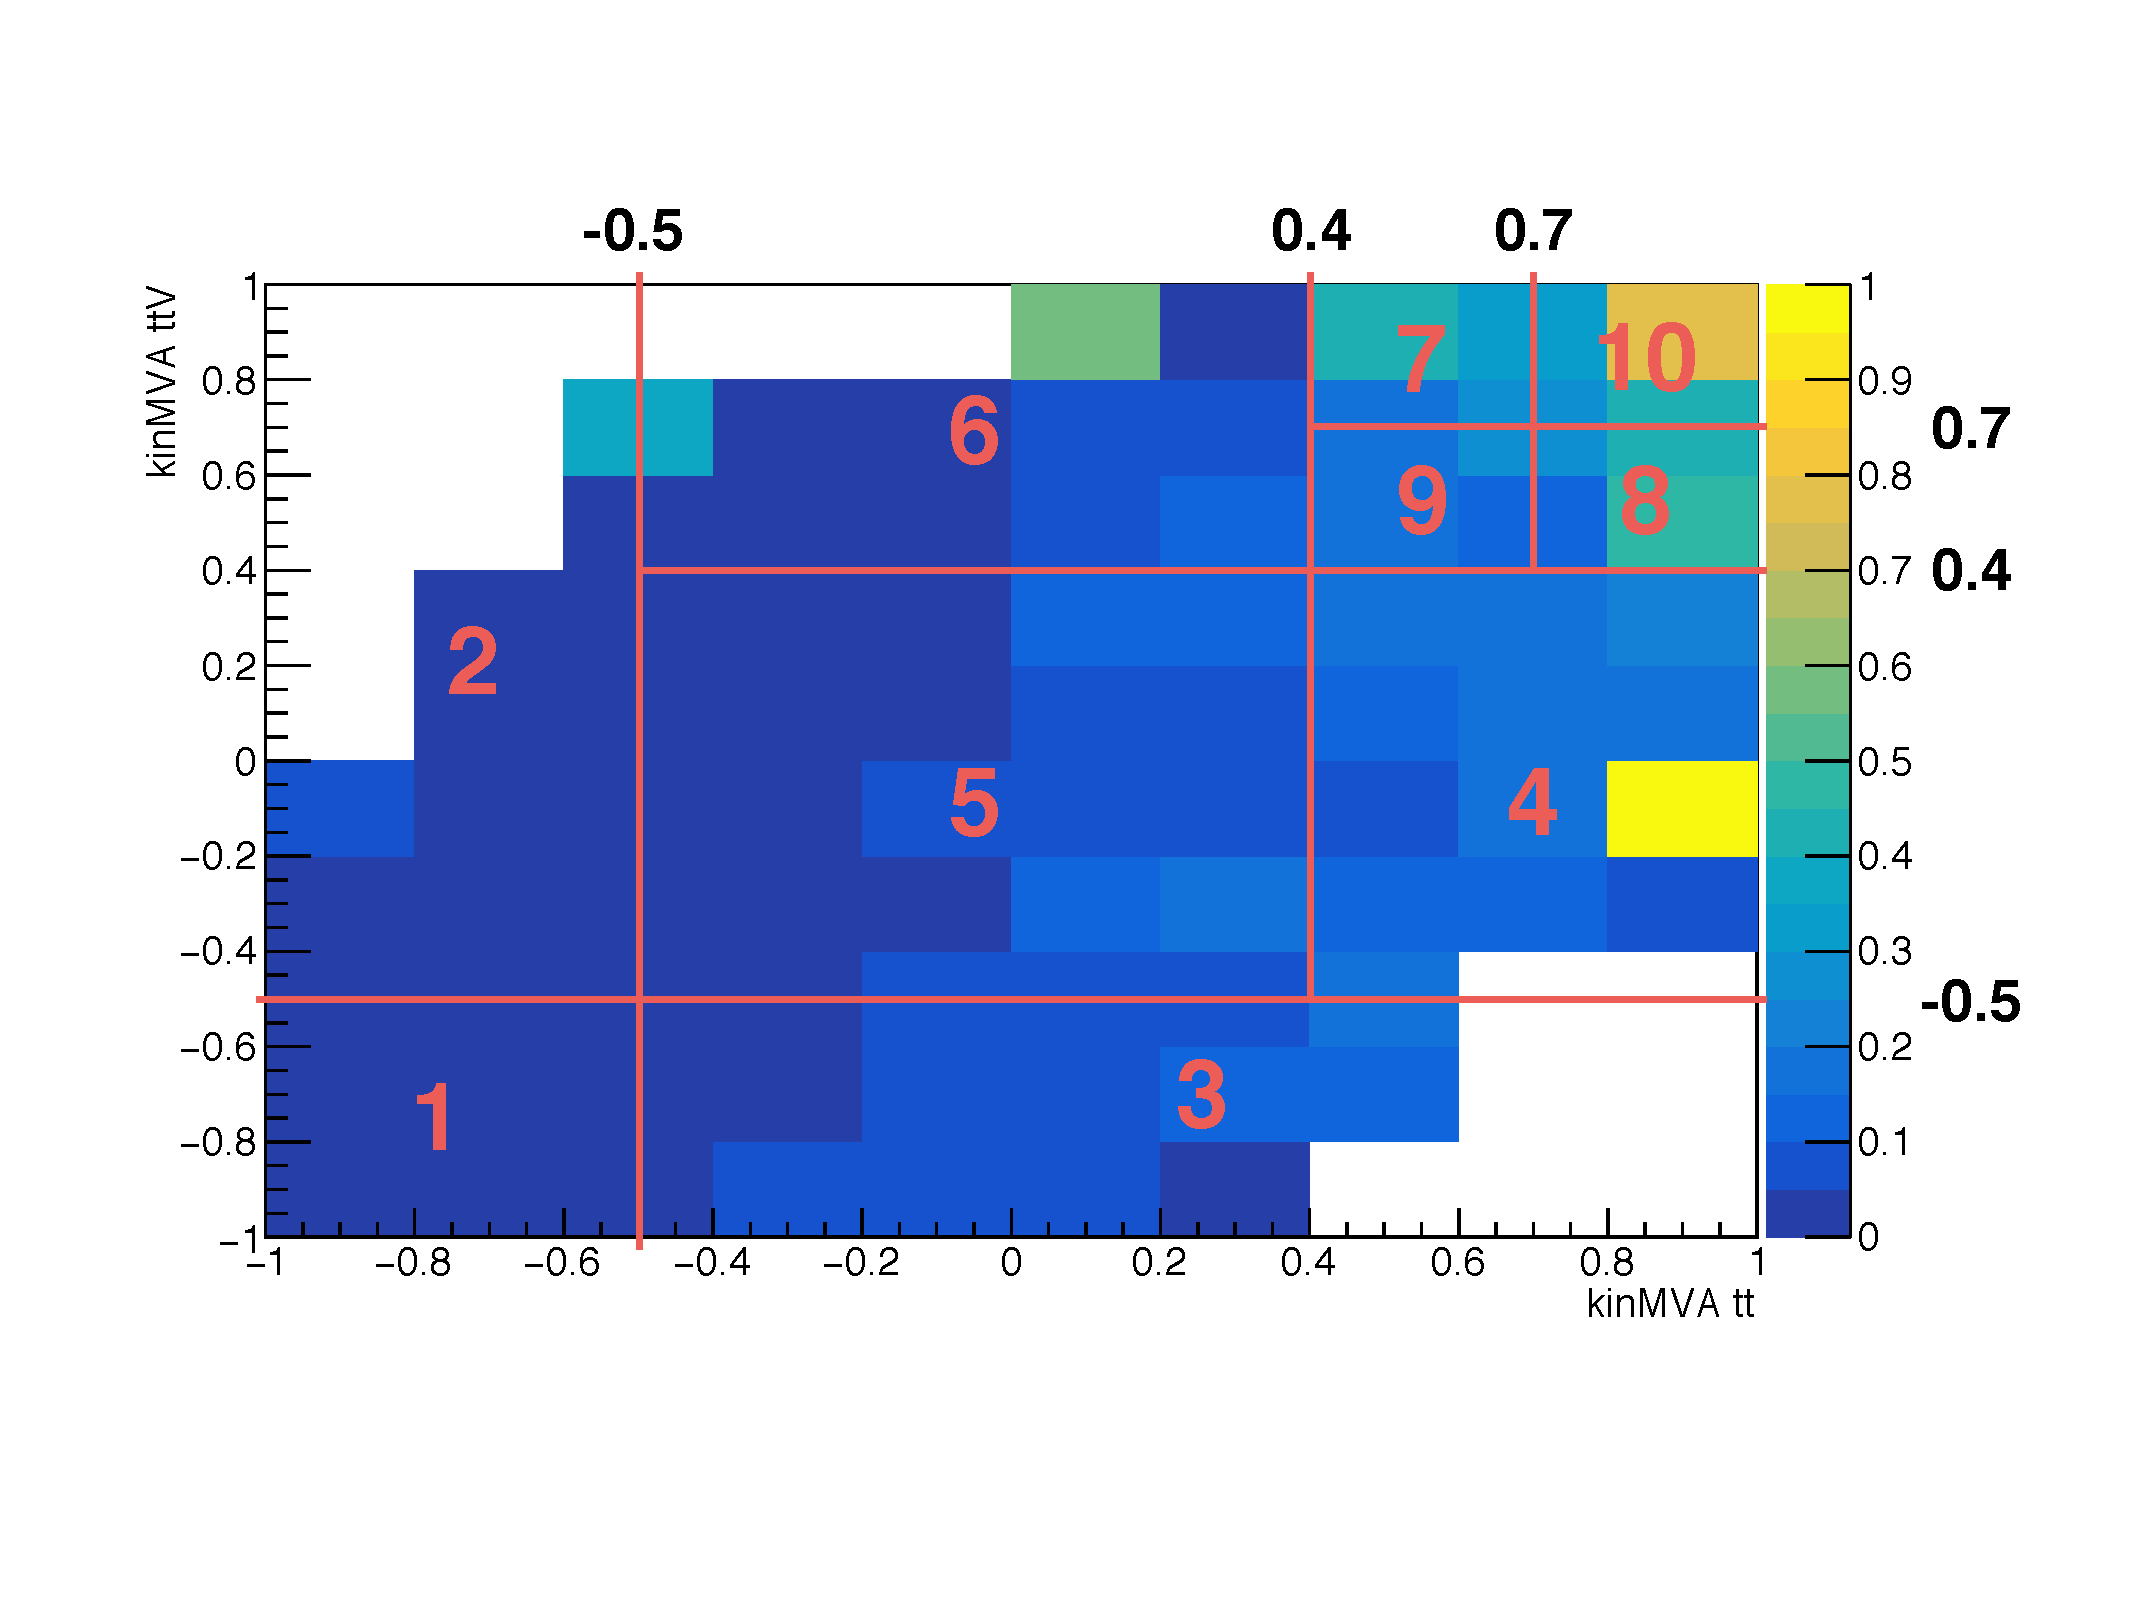
\includegraphics[width=0.8\textwidth]{figures/hratio_binning.pdf}
\caption{Binning overlaid on the S/B ratio map on the plane of classifier outputs.}
\label{fig:binning}
\end{figure}

From this event categorization, a 1D histogram of expected distribution is produced for each signal and background process, and fit to the observed data (or the Asimov dataset for expected limits).

\subsection{Signal model}
The goal of this analysis is to test the compatibility of points in the parameter space of Higgs-to-vector boson and Higgs-to-top quark couplings.
The simulated \tHq, \tHW, and \ttH\ signal events are used with event-by-event weights to reflect the impact of the couplings on kinematic distributions, and together with different predictions of the respective production cross sections and branching ratios, we can produce limits for different values of \CV\ and \Ct.
(See Tab.~\ref{tab:reweight} for the set of \Ct\ and \CV\ values generated.)
The slight shape-dependence of the BDT outputs as a function of the couplings is documented in App.~\ref{sec:bdtvscvct}.

Apart from the \Ct/\CV\ interference of the \tHq\ and \tHW\ production cross sections, the cross section of \ttH\ scales as $\Ct^2$.
Furthermore, the Higgs branching fractions to vector bosons depend on \CV, and the overall Higgs decay width depend both on \Ct\ and \CV\ when considering resolved top-quark loops in the $\PH\to\gamma\gamma$, $\PH\to\Z\gamma$, and $\PH\to\Pg\Pg$ decays.
The relative contributions from $\PH\to\WW$, $\PH\to\ZZ$, and $\PH\to\tautau$ changes with changing \CV.

We hence set an upper limit on the combined cross section times branching ratio of \tHq, \tHW, and \ttH.

If we assume a modifier for the Higgs-to-tau coupling ($\kappa_\tau$) to be equal to $\Ct$, the relative fractions of $\WW$, $\ZZ$, and $\tautau$ in our selection will only depend on the ratio of $\Ct/\CV$.
Any limit set at any given value of $\Ct/\CV$ is thus valid for all values of $\Ct$ and $\CV$ with that ratio, and could then be compared with theoretical predictions of cross sections at different values of either modifier.
Rather than as a function of the $\Ct/\CV$ ratio, limits could (equivalently) be reported as a function of the relative strength of Higgs-top and Higgs-vector-boson couplings, multiplied by the relative sign.
Such a parameter, further referred to as \ft, as defined in Eq.~\ref{eq:ft}, spans the entire possible parameter space between $-1.0$ and $1.0$, with the SM expectation at $0.5$.
Absolute values of $1.0$ or $0.0$ would then correspond to purely Higgs-top and purely Higgs-V couplings, respectively.
\begin{equation} \label{eq:ft}
	\ft = \mathrm{sign}(\Ct/\CV) \times \frac{\Ct^2}{\Ct^2+\CV^2}.
\end{equation}

Table~\ref{tab:ctcvvalues} shows the points in the $\Ct/\CV$ and \ft\ parameter space that are mapped by the 51 individual \Ct\ and \CV\ points.

\begin{table}[h!]
\centering
\begin{tabular}{rrrrr}
 $\ft$ & \Ct/\CV & $\CV=0.5$ & $\CV=1.0$ & $\CV=1.5$ \\ \hline
  -0.973 & -6.000 & -3.00 &       &       \\
  -0.941 & -4.000 & -2.00 &       &       \\
  -0.900 & -3.000 & -1.50 & -3.00 &       \\
  -0.862 & -2.500 & -1.25 &       &       \\
  -0.800 & -2.000 & -1.00 & -2.00 & -3.00 \\
  -0.692 & -1.500 & -0.75 & -1.50 &       \\
  -0.640 & -1.333 &       &       & -2.00 \\
  -0.610 & -1.250 &       & -1.25 &       \\
  -0.500 & -1.000 & -0.50 & -1.00 & -1.50 \\
  -0.410 & -0.833 &       &       & -1.25 \\
  -0.360 & -0.750 &       & -0.75 &       \\
  -0.308 & -0.667 &       &       & -1.00 \\
  -0.200 & -0.500 & -0.25 & -0.50 & -0.75 \\
  -0.100 & -0.333 &       &       & -0.50 \\
  -0.059 & -0.250 &       & -0.25 &       \\
  -0.027 & -0.167 &       &       & -0.25 \\
   0.000 &  0.000 &  0.00 &  0.00 &  0.00 \\
   0.027 &  0.167 &       &       &  0.25 \\
   0.059 &  0.250 &       &  0.25 &       \\
   0.100 &  0.333 &       &       &  0.50 \\
   0.200 &  0.500 &  0.25 &  0.50 &  0.75 \\
   0.308 &  0.667 &       &       &  1.00 \\
   0.360 &  0.750 &       &  0.75 &       \\
   0.410 &  0.833 &       &       &  1.25 \\
   0.500 &  1.000 &  0.50 &  1.00 &  1.50 \\
   0.610 &  1.250 &       &  1.25 &       \\
   0.640 &  1.333 &       &       &  2.00 \\
   0.692 &  1.500 &  0.75 &  1.50 &       \\
   0.800 &  2.000 &  1.00 &  2.00 &  3.00 \\
   0.862 &  2.500 &  1.25 &       &       \\
   0.900 &  3.000 &  1.50 &  3.00 &       \\
   0.941 &  4.000 &  2.00 &       &       \\
   0.973 &  6.000 &  3.00 &       &       \\ \hline
\end{tabular}
\caption{The 33 distinct values of $\Ct/\CV$ and \ft\ as mapped by the 51 \Ct\ and \CV\ points.}
\label{tab:ctcvvalues}
\end{table}

The overall higgs decay width (modified by both \Ct\ and \CV) becomes irrelevant if limits are quoted as absolute cross sections rather than multiples of the expected cross section (which depends on the overall Higgs decay width).

% Two possibilities are explored: one where the $\gamma\gamma$, $\Z\gamma$, and $\Pg\Pg$ decays are modified with \Ct\ (referred to as the ``resolved'' model henceforth), and one where they are kept fixed at their SM values.
% In both cases, the $\PH\to\cPqc\cPqc$ branching is left unchanged with \Ct.

The 1D histograms of events as categorized in regions of the 2D BDT plane is then used in a maximum likelihood fit of signal and background shapes, where the \tHq, \tHW, and \ttH\ signals are floating with a common signal strength modifier $r$, producing a 95\% C.L. upper limit the observed cross section of $\tHq+\tHW+\ttH$.

This is done separately for each point of \Ct\ and \CV, where the cross sections and branching fractions are scaled accordingly in each point.
Limits at fixed values of $\Ct/\CV$ are by construction identical.
Tables~\ref{tab:brscalingK6_0p5}--\ref{tab:brscalingK6_1p5} and~\ref{tab:xsbrscalingK6_0p5}--\ref{tab:xsbrscalingK6_1p5} in Appendix~\ref{sec:xsbrscalings} show the scalings of cross section times branching fraction, as well as branching fractions alone for each of the Higgs decay modes and each of the signal components.

%% Leaving out the limit plots in each channel for now.
% \begin{figure} [!h]
%  \centering
%  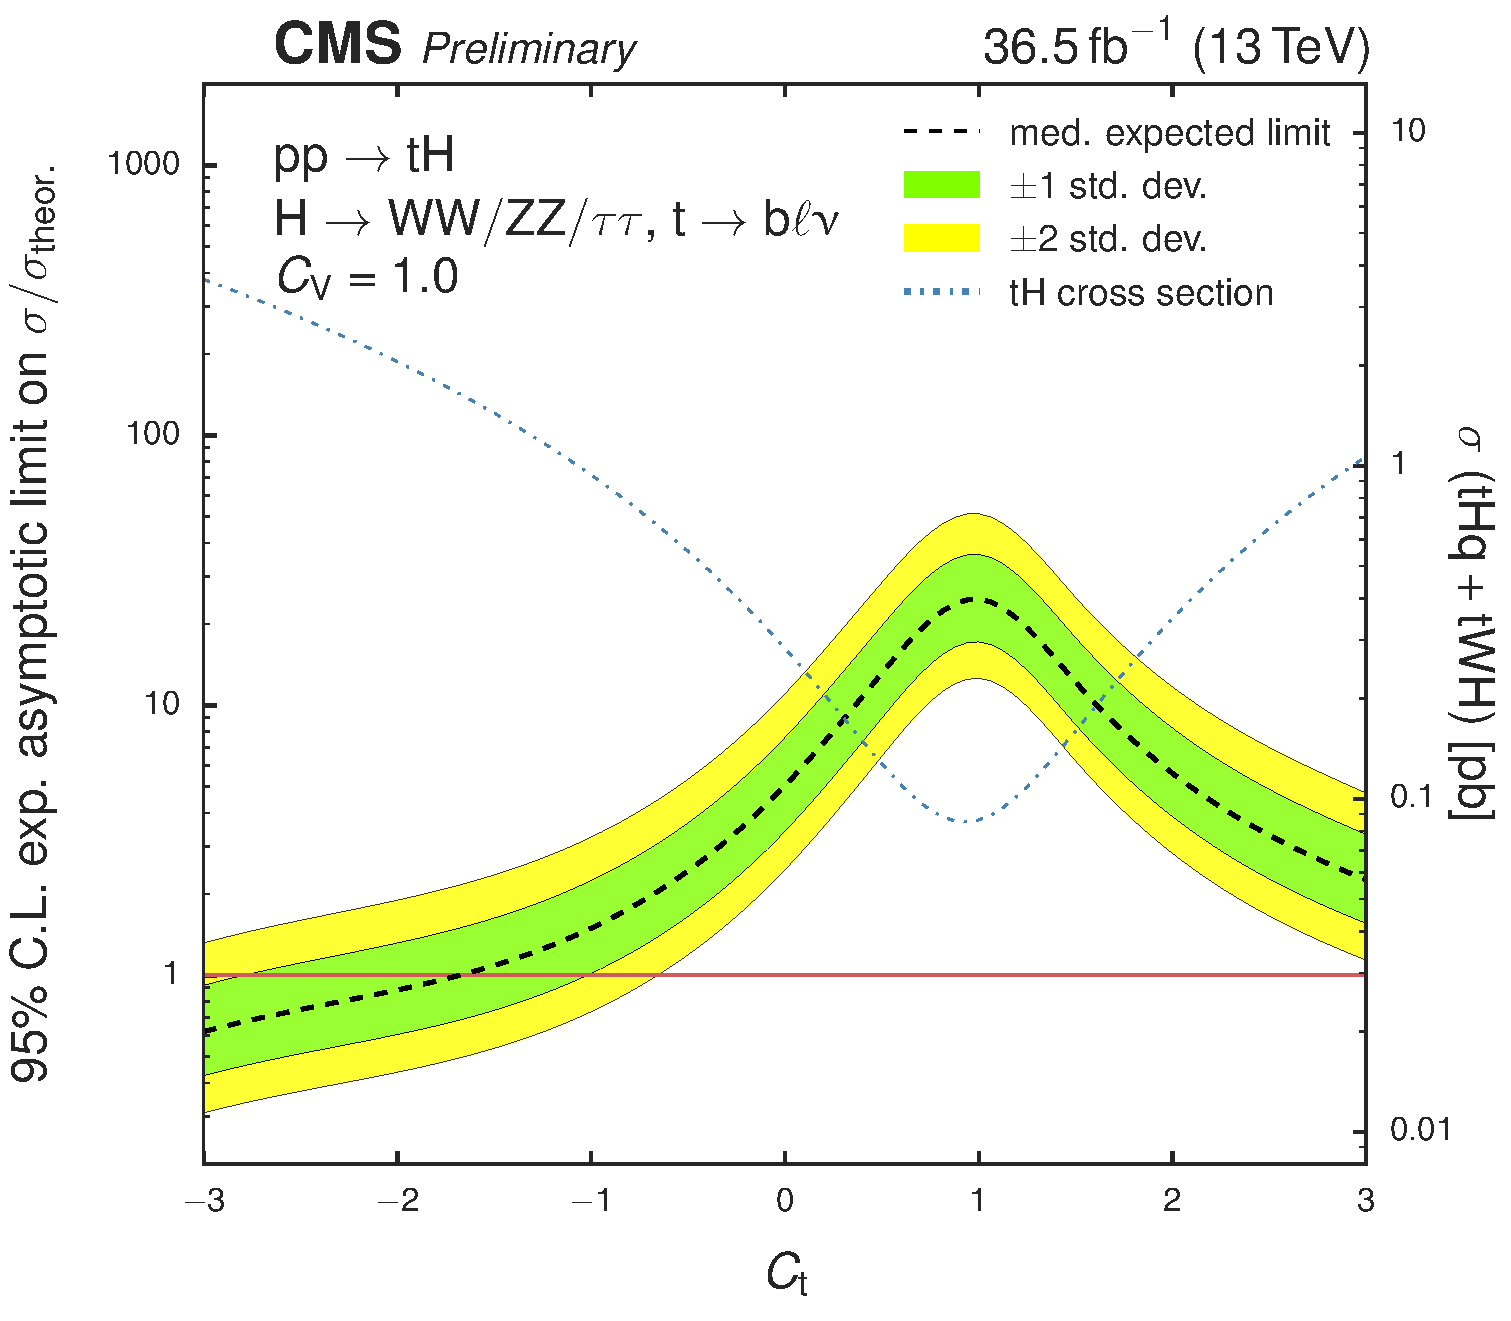
\includegraphics[width=0.32\textwidth]{figures/limits/limits_3l_cv_1p0.pdf}
%  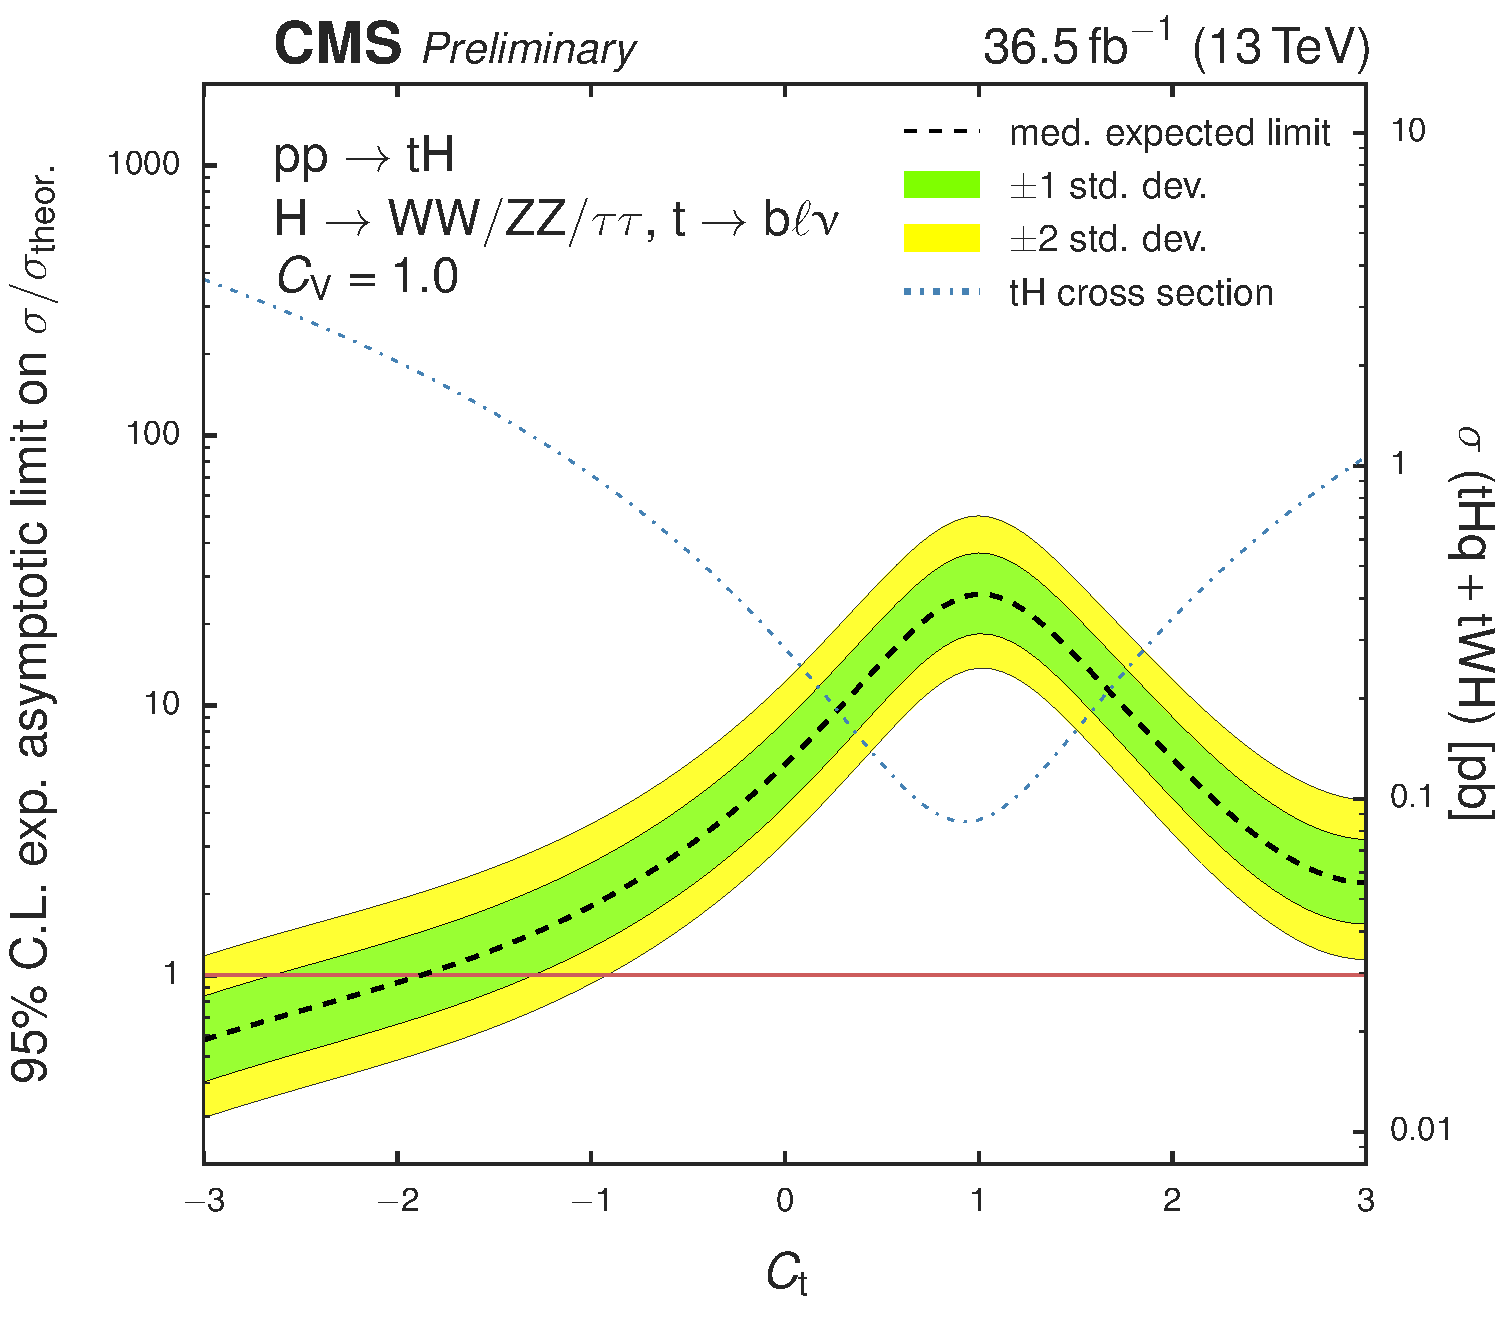
\includegraphics[width=0.32\textwidth]{figures/limits/limits_2lss_mm_cv_1p0.pdf}
%  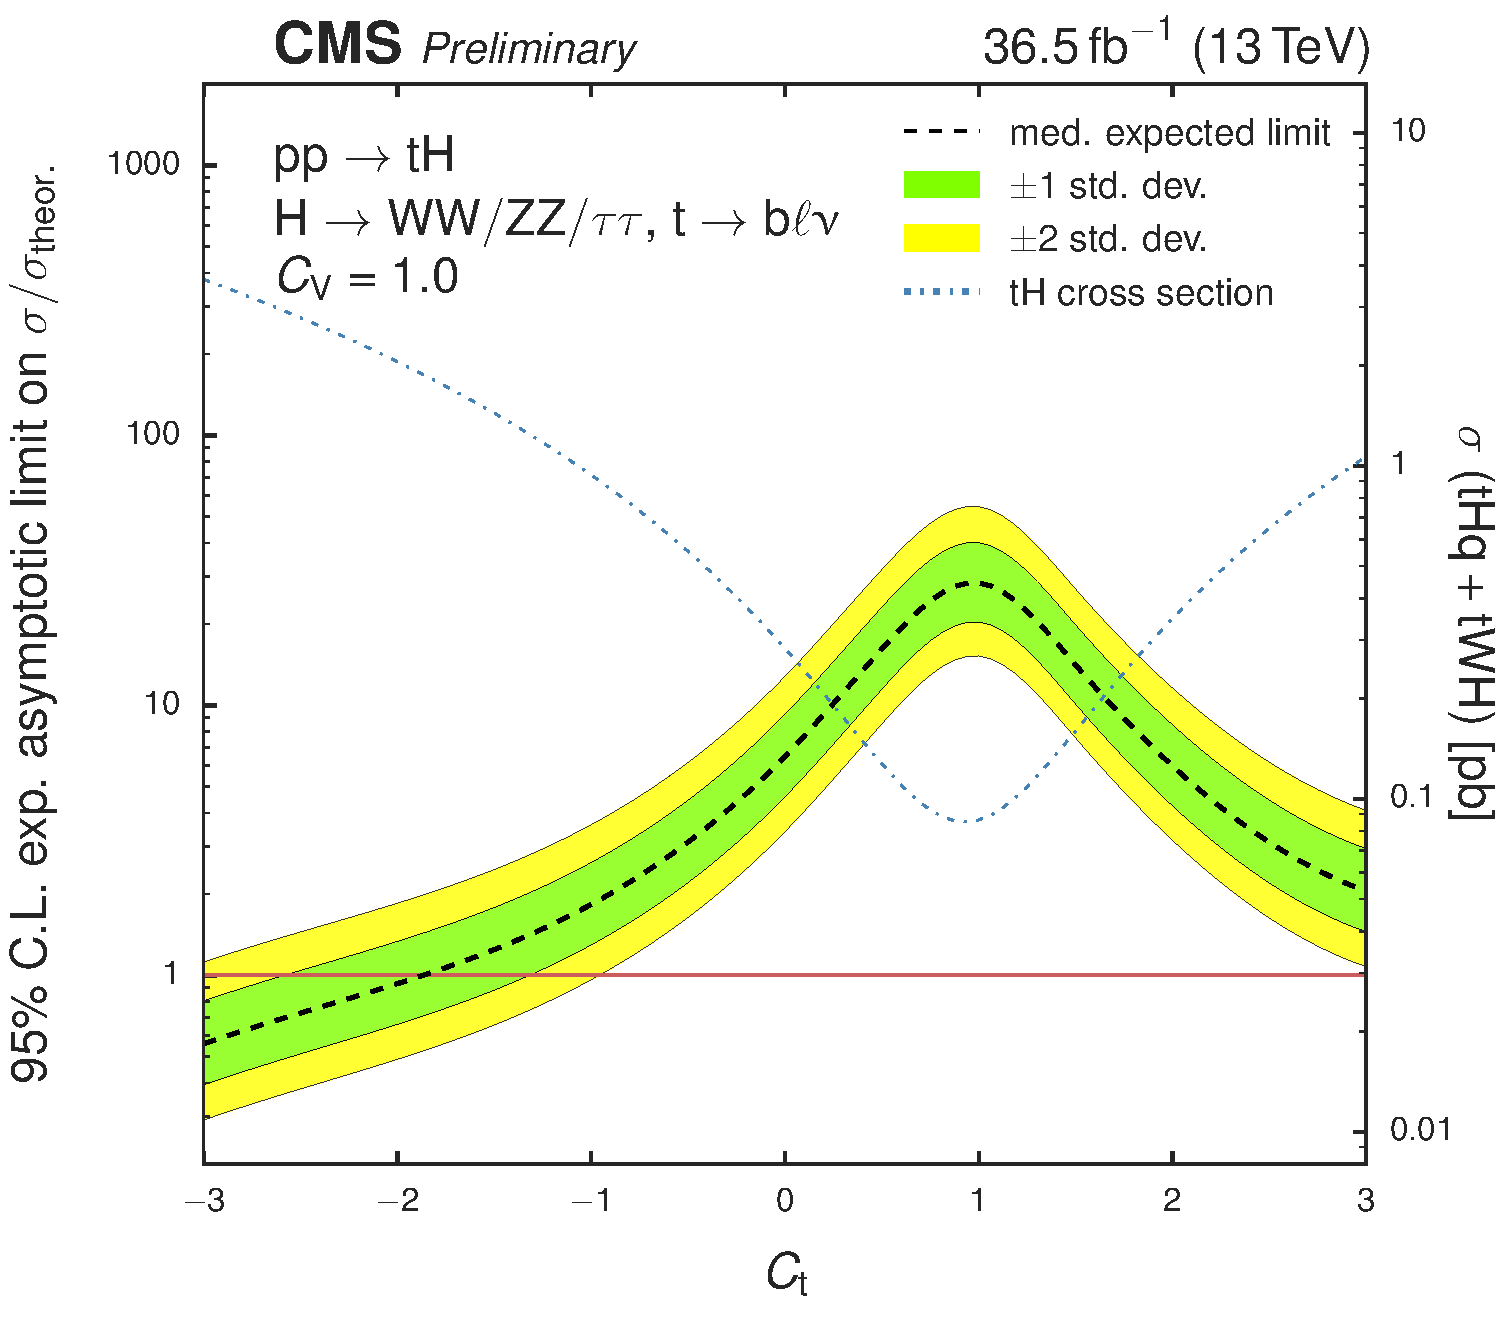
\includegraphics[width=0.32\textwidth]{figures/limits/limits_2lss_em_cv_1p0.pdf} \\
%  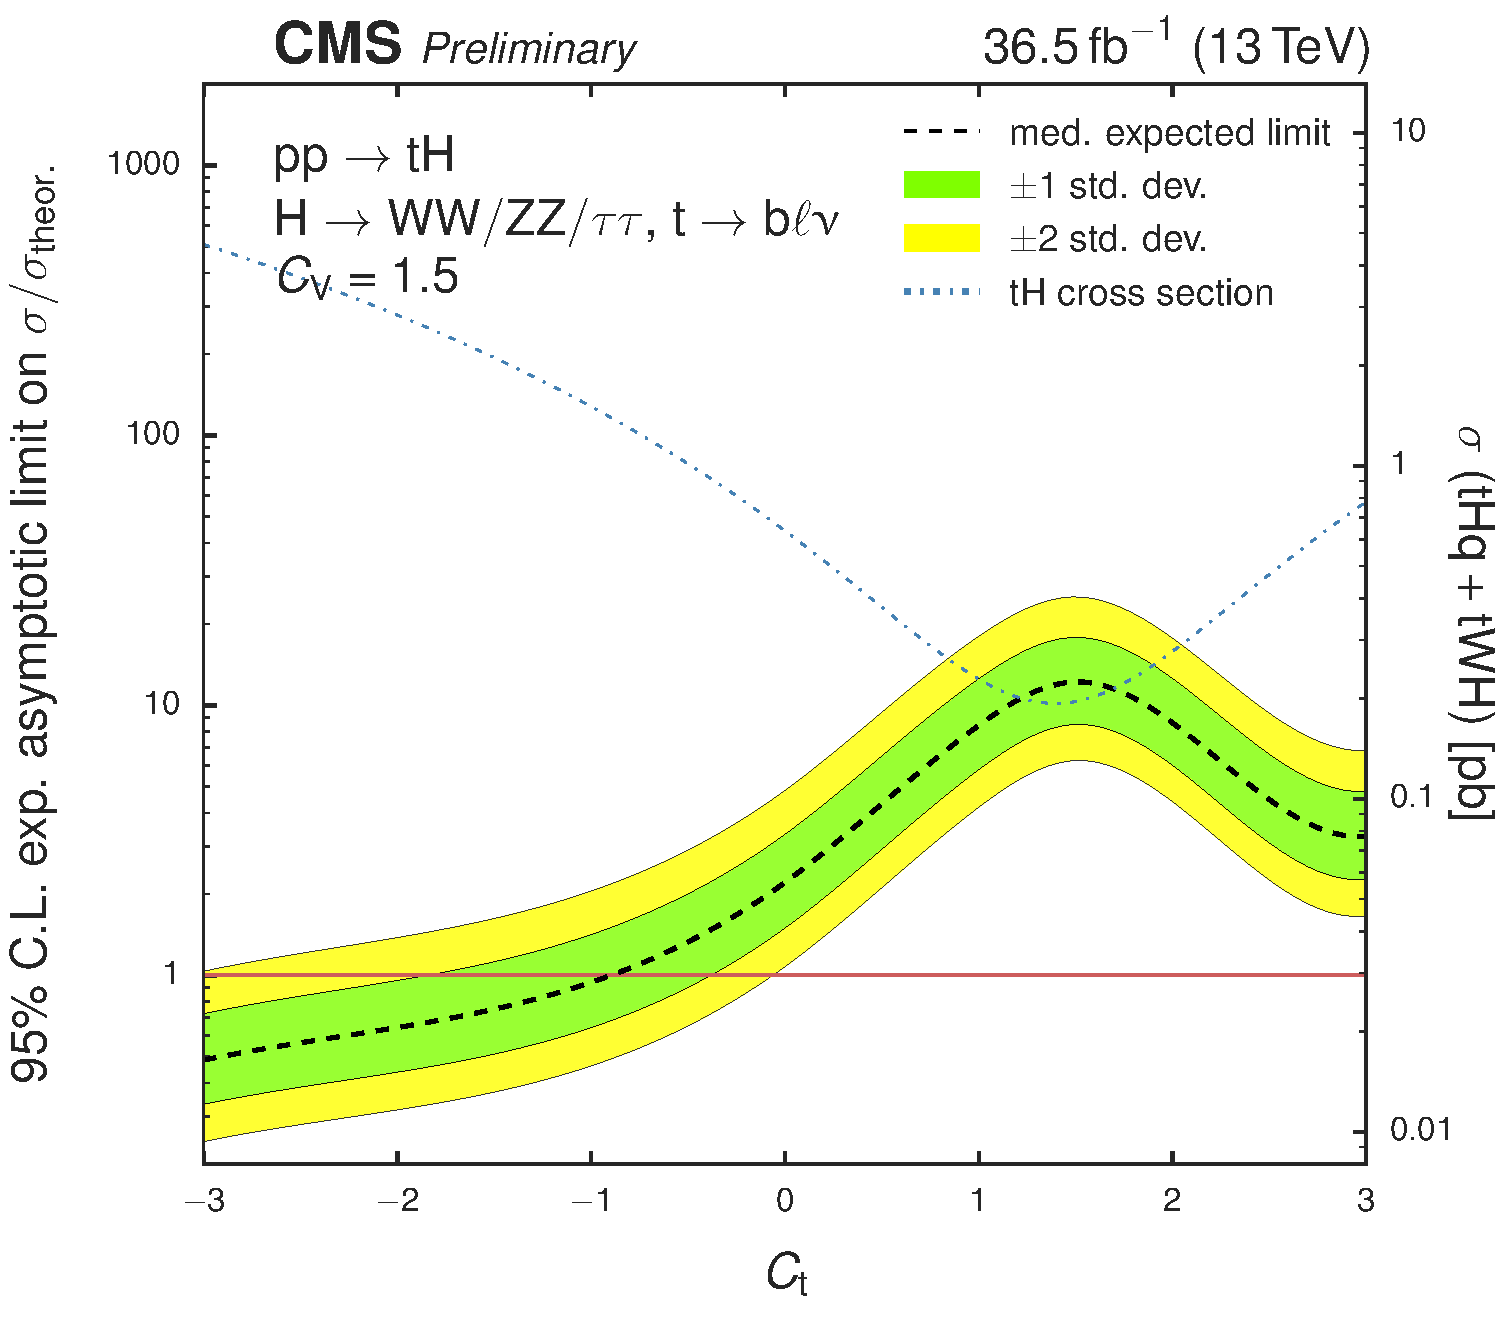
\includegraphics[width=0.32\textwidth]{figures/limits/limits_3l_cv_1p5.pdf}
%  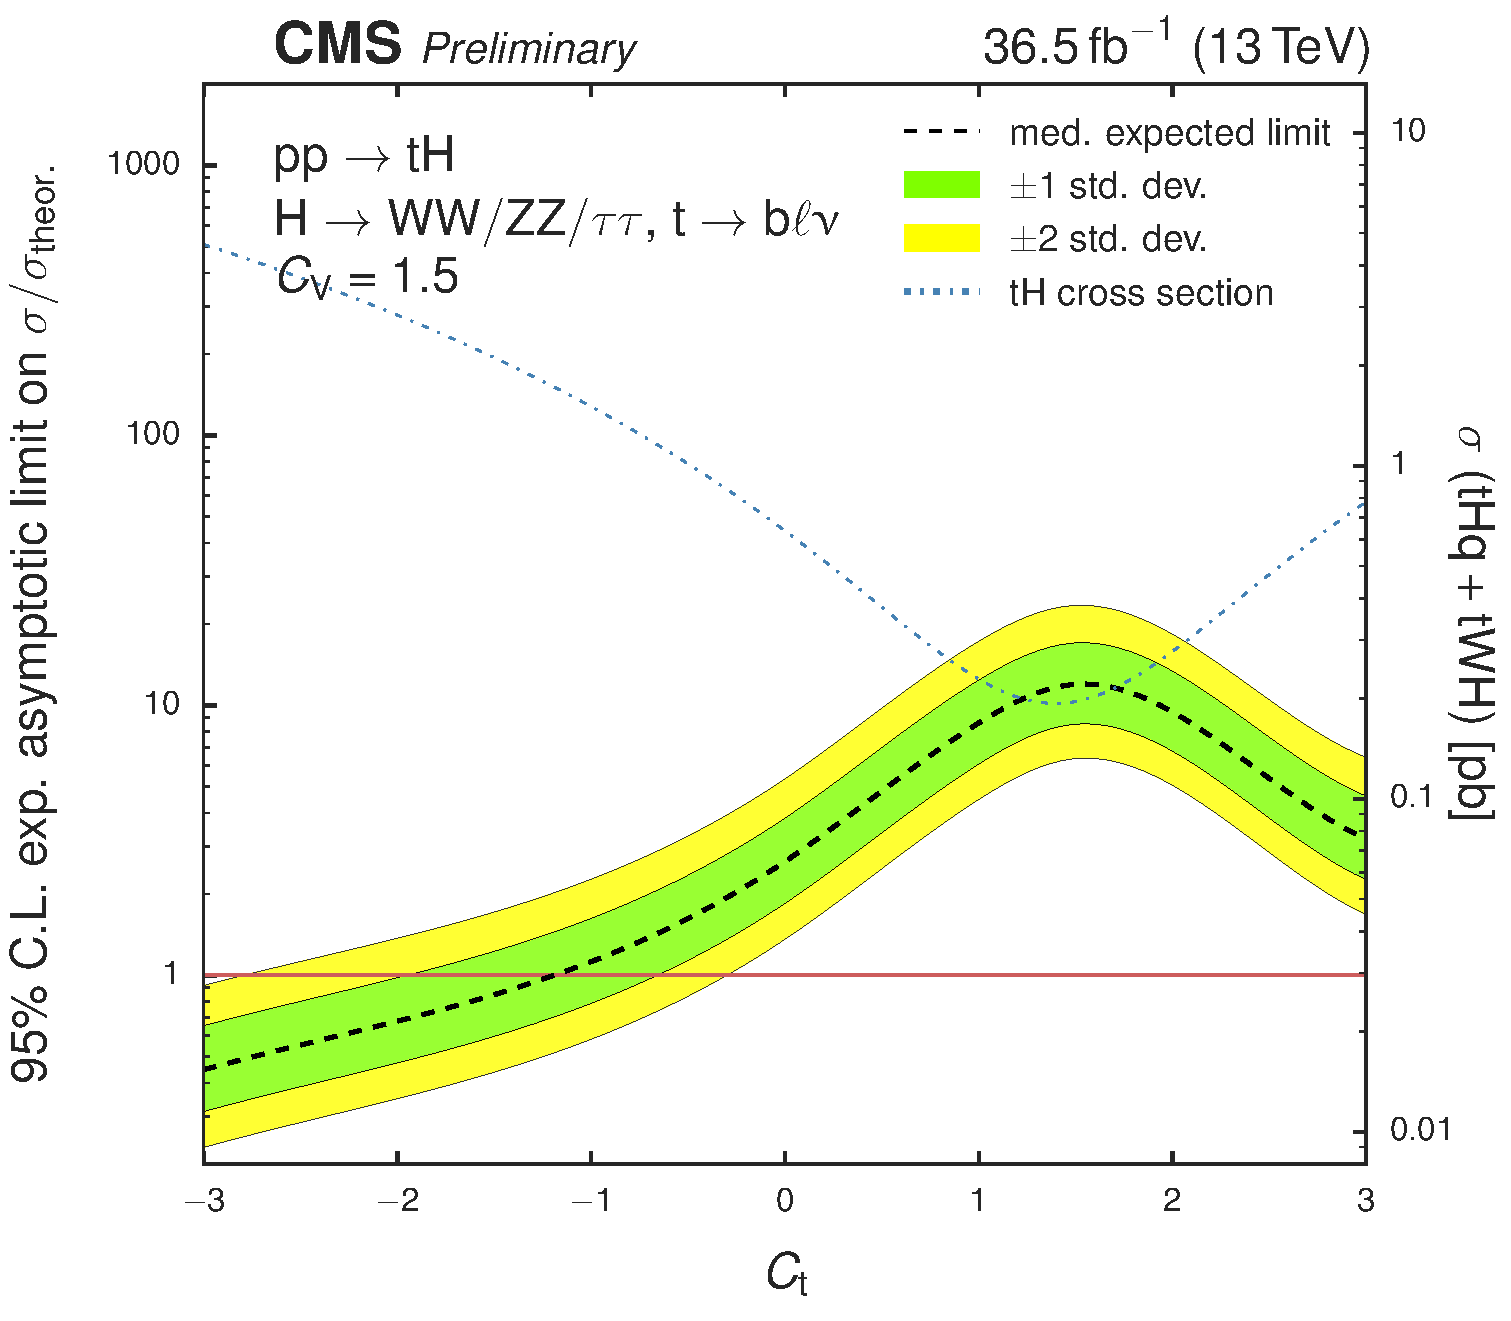
\includegraphics[width=0.32\textwidth]{figures/limits/limits_2lss_mm_cv_1p5.pdf}
%  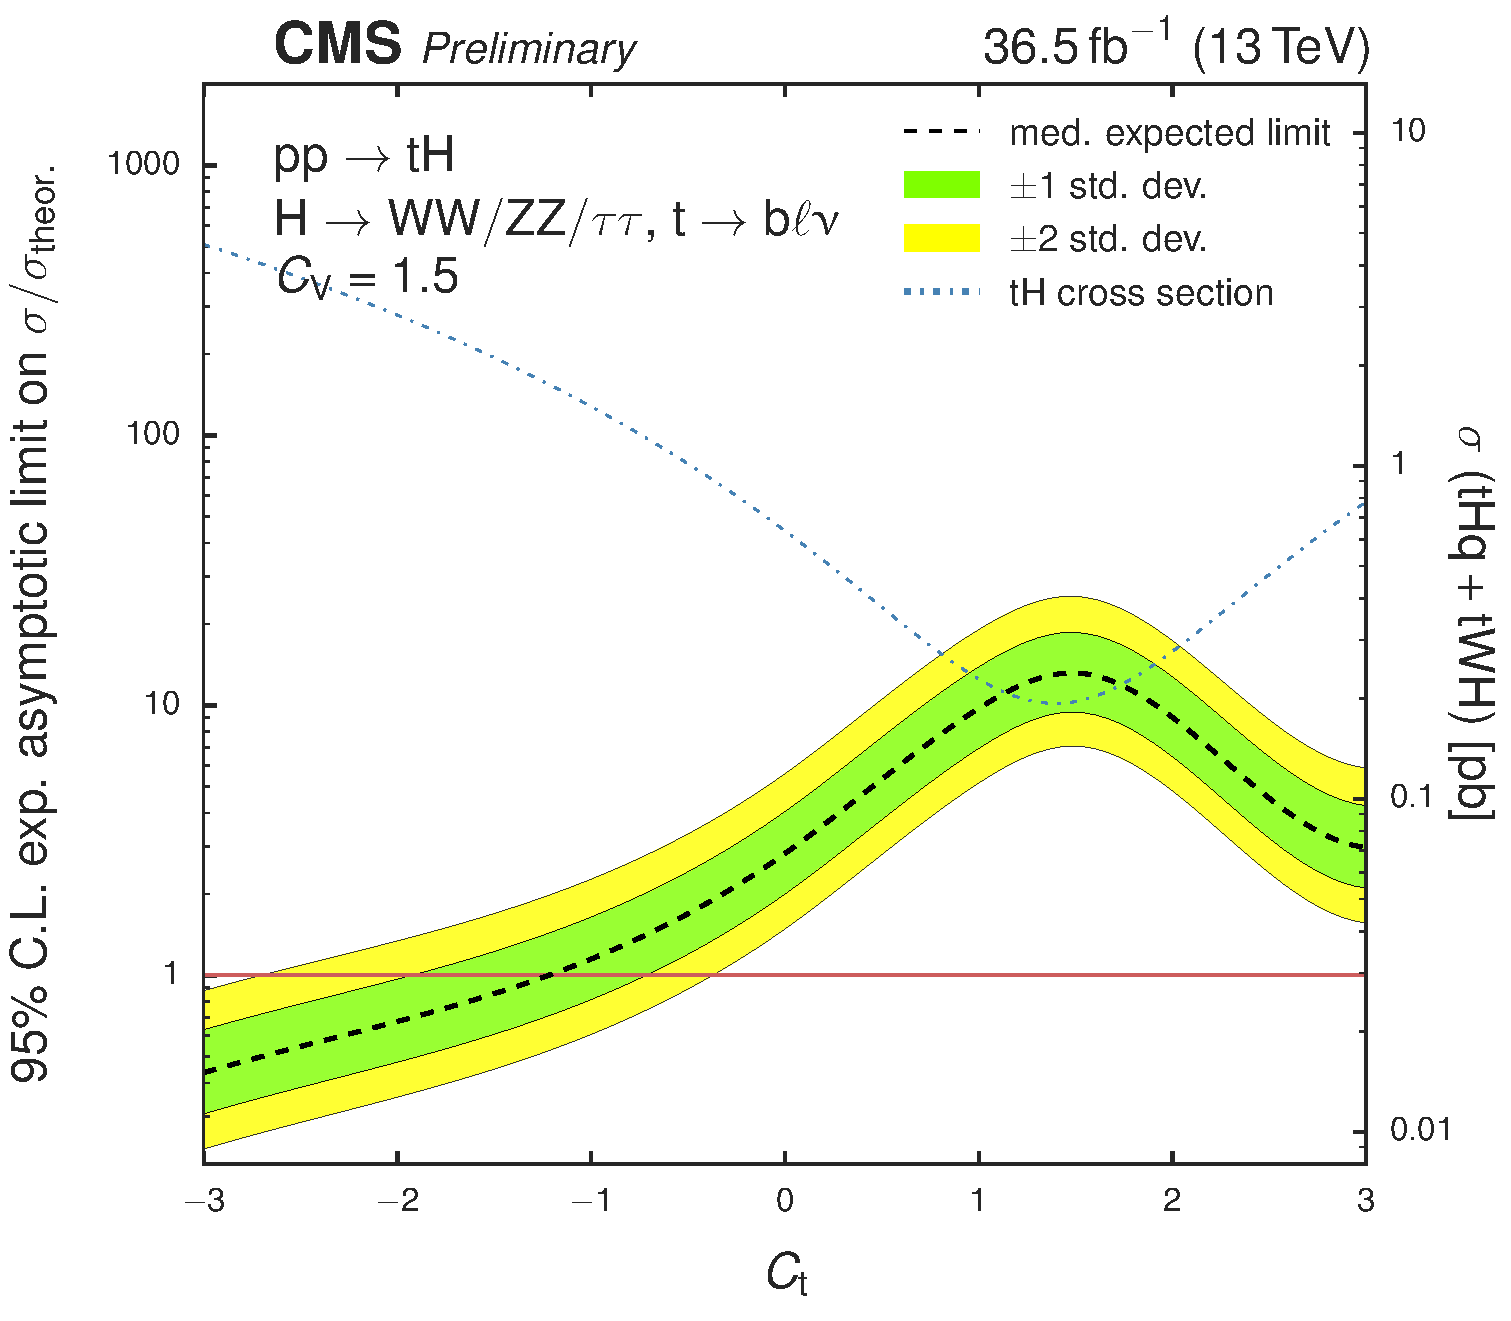
\includegraphics[width=0.32\textwidth]{figures/limits/limits_2lss_em_cv_1p5.pdf} \\
%  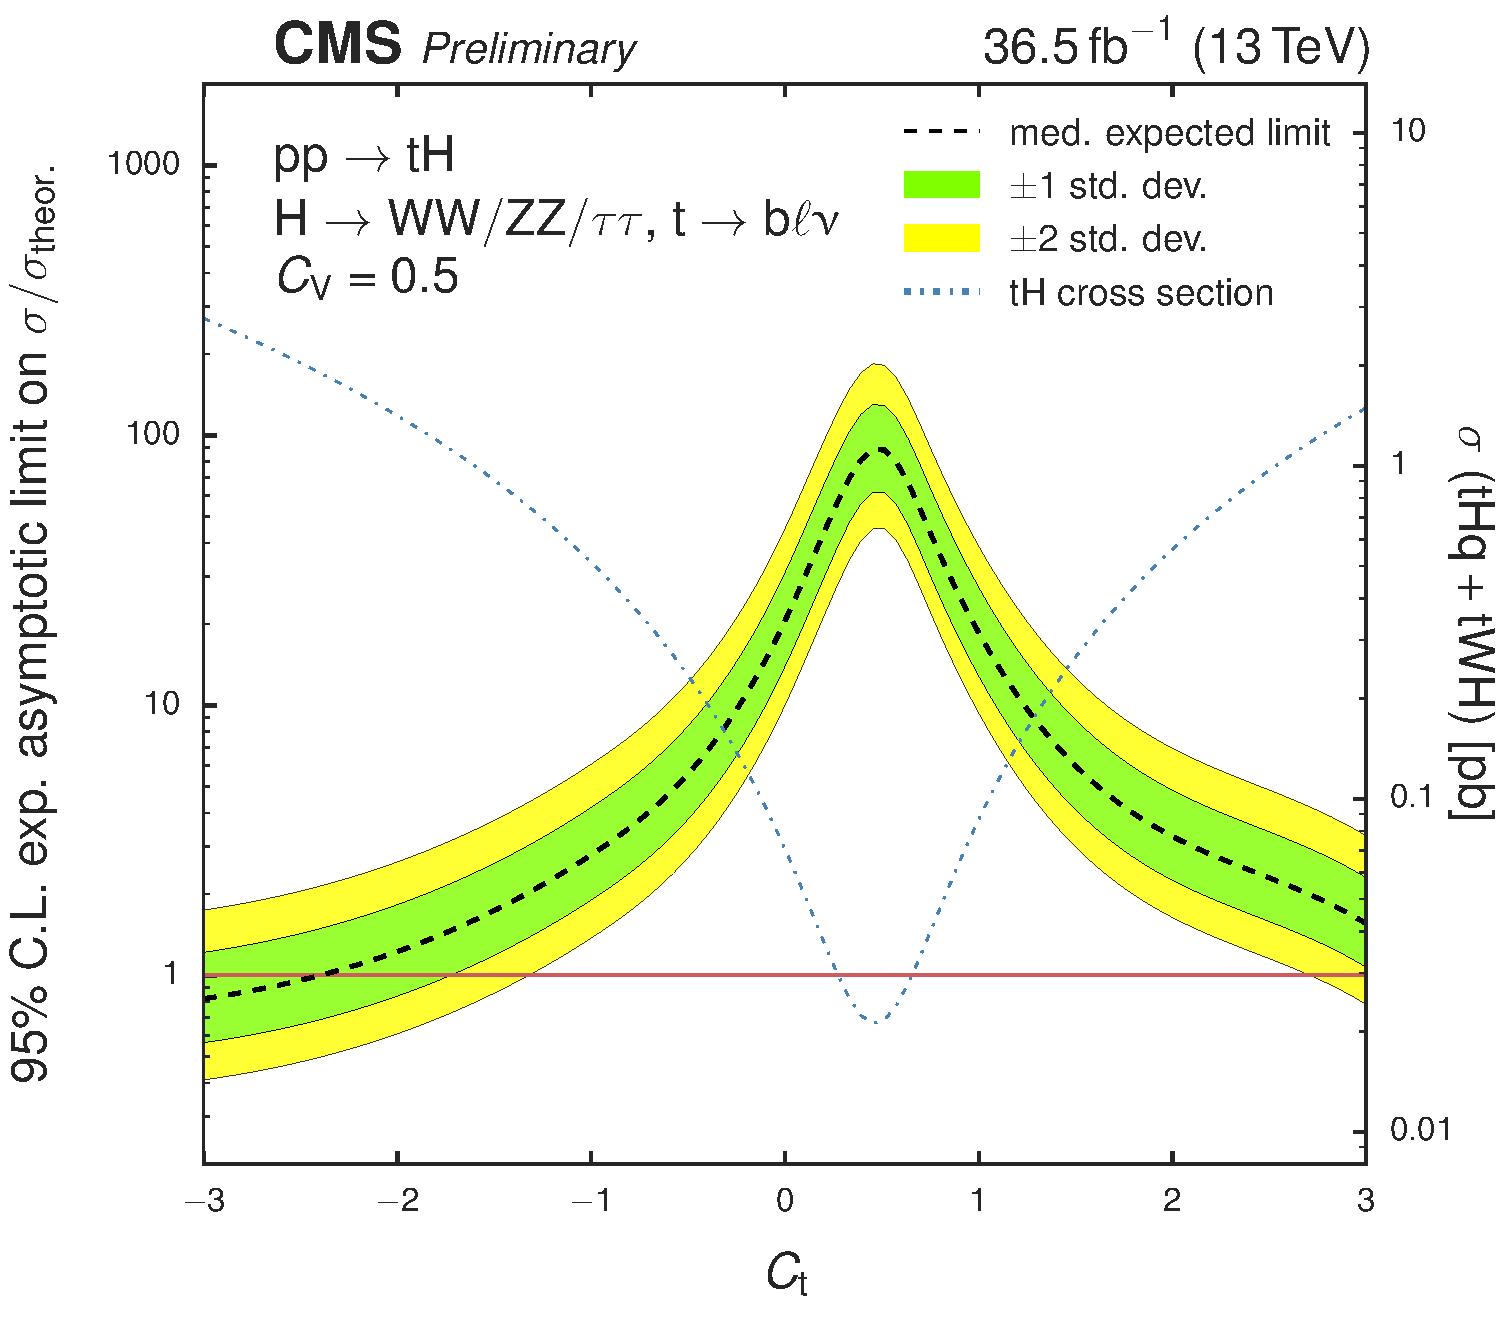
\includegraphics[width=0.32\textwidth]{figures/limits/limits_3l_cv_0p5.pdf}
%  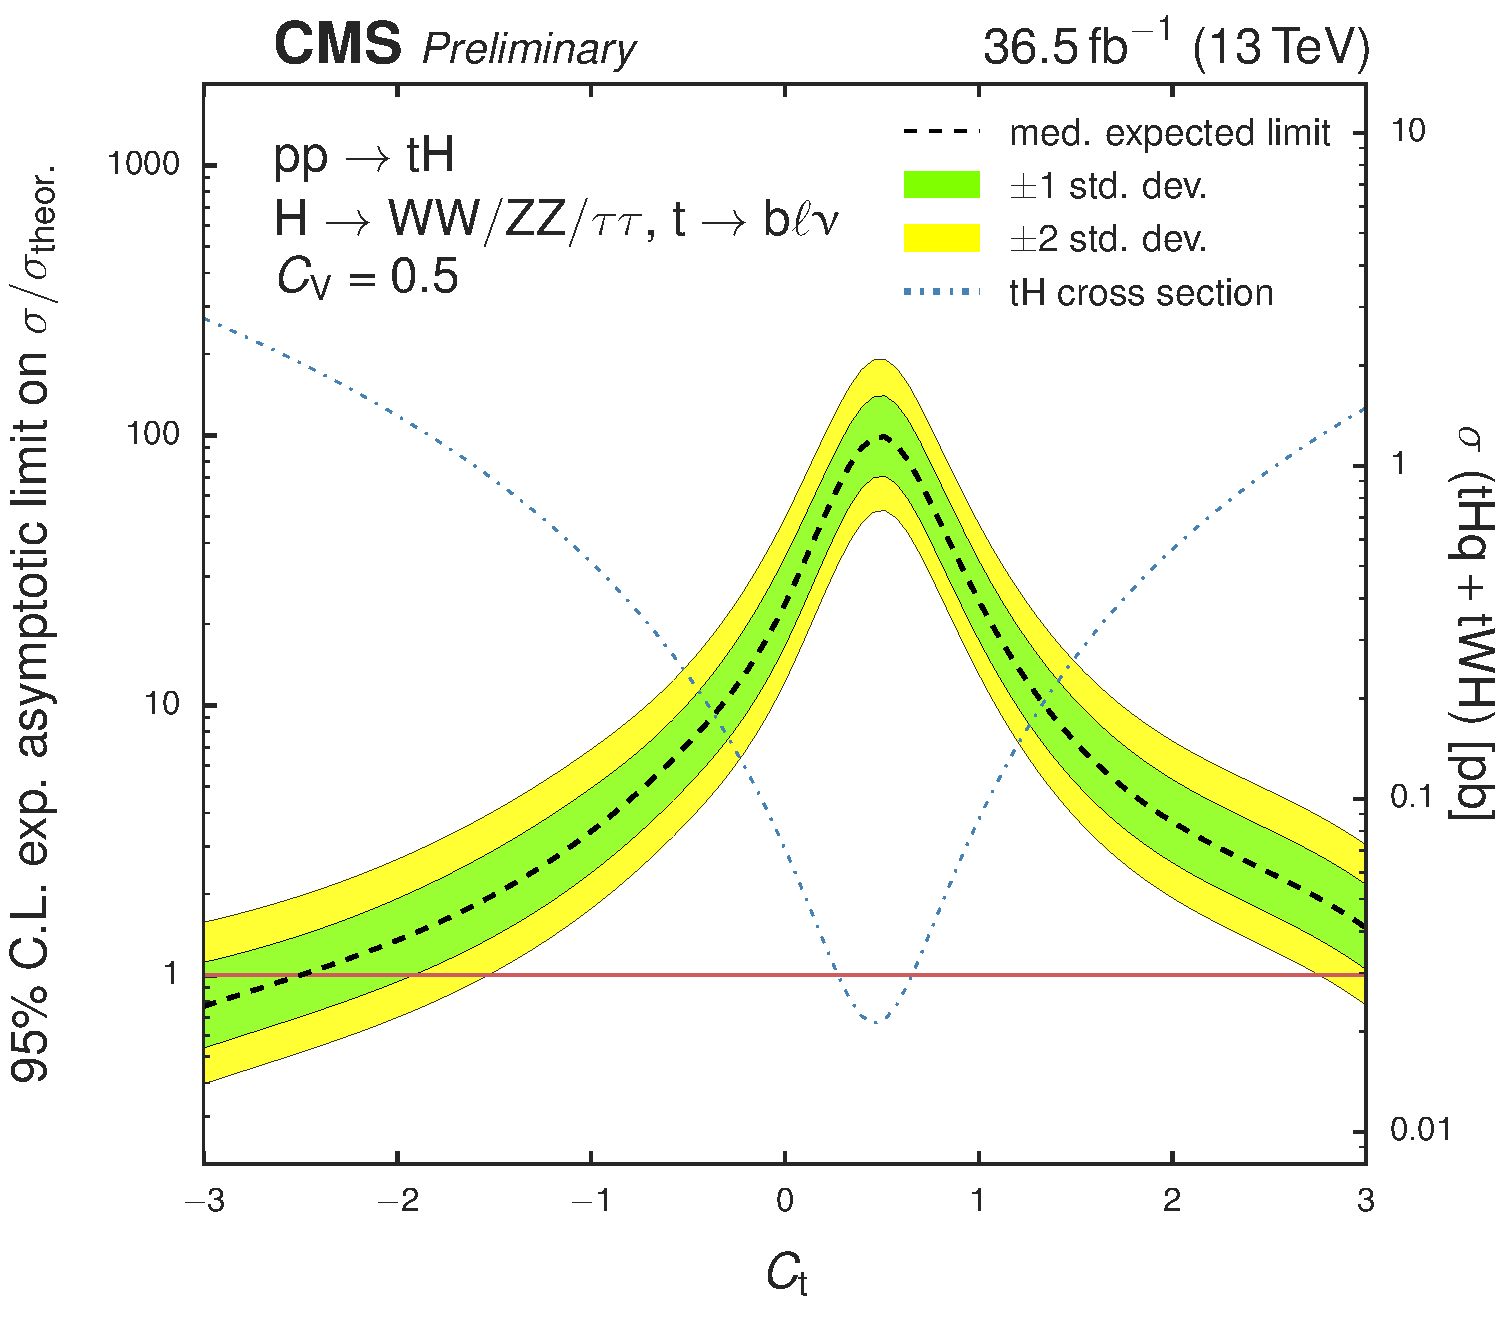
\includegraphics[width=0.32\textwidth]{figures/limits/limits_2lss_mm_cv_0p5.pdf}
%  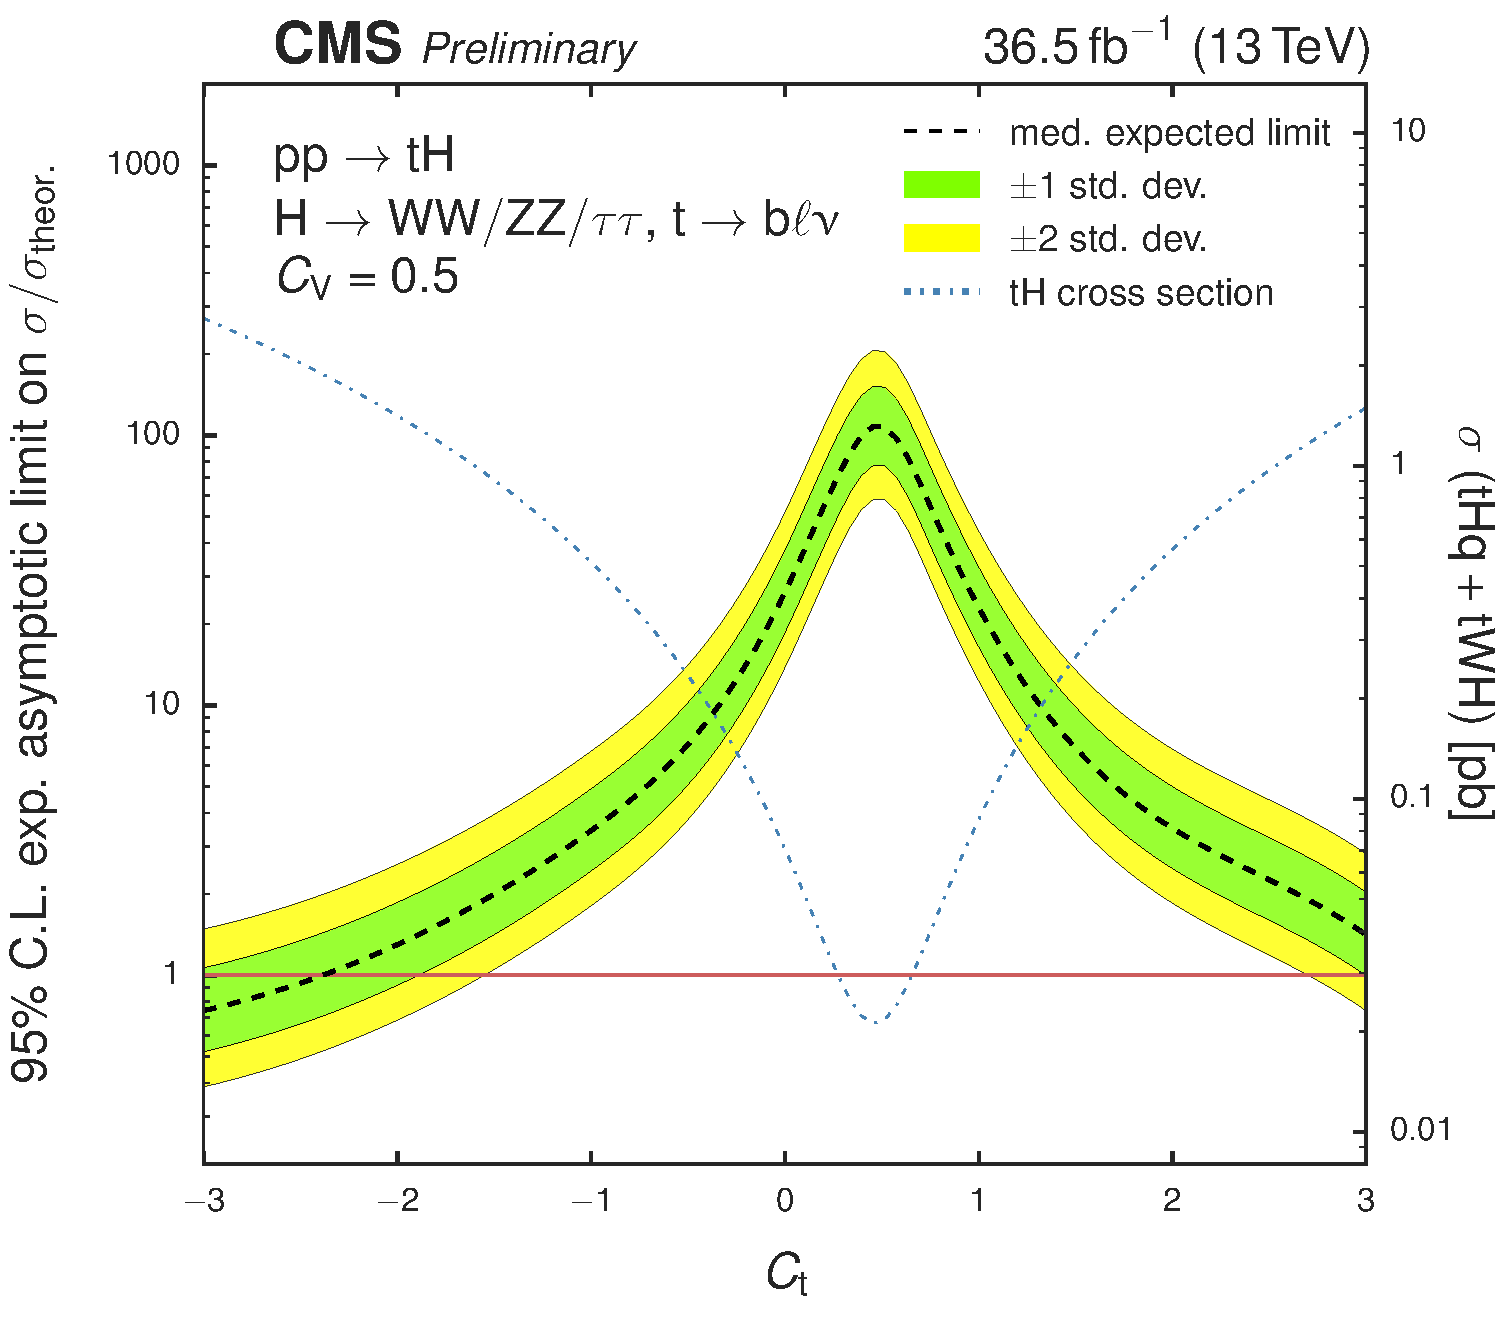
\includegraphics[width=0.32\textwidth]{figures/limits/limits_2lss_em_cv_0p5.pdf}
% \
% \caption{Expected asymptotic limit on $\frac{\sigma}{\sigma_{theor}}$ as a function of \Ct\ for $\CV=1.0$, $\CV=1.5$, $\CV=0.5$ (top to bottom) for the three lepton channel (left), the \mumu\ channel (middle), and the \emu\ channel (right).}
% \label{fig:limits_cv_3l}
% \end{figure}



